\section{Xamarin.Forms: 3 Native UIs, 1 Shared Code Basis}
Bei Xamarin.Forms handelt es sich um ein .NET-basiertes UI Toolkit, mit dem Oberfl�chen entweder in
C\# oder einem speziellen XAML-Dialekt generisch definiert werden.W�hrend des Kompiliervorgangs
entstehen aus dem Code plattformspezifische, native Oberfl�chen. Xamarin.Forms unterst�tzt die
Plattformen iOS, Android und Windows Phone, aber (noch) nicht Windows Store Apps. Mit Xamarin.Forms
k�nnen Entwickler deutlich weniger Code schreiben.
Ziel dieser Arbeit ist speziell Xamarin.Forms zu untersuchen.

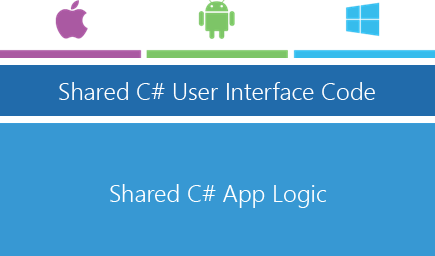
\includegraphics[scale = 0.5]{graphics/XamarinForms1.png}
\\Eine Beispiel Solution sehen wir in der folgenden Abbildung: 

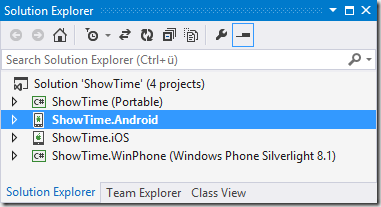
\includegraphics[scale = 0.5]{graphics/xamarin_forms-solution.png}
\\Die gemeinsame Gesch�ftslogik ist in der Portable Class Library beinhaltet. Zus�tzlich werden noch
drei weitere Projekte erstellt, eins f�r Android, eins f�r iOS und eins f�r Windows Phone. In den
plattformspezifischen Projekte befinden sich plattformspezifische Views und Logik.

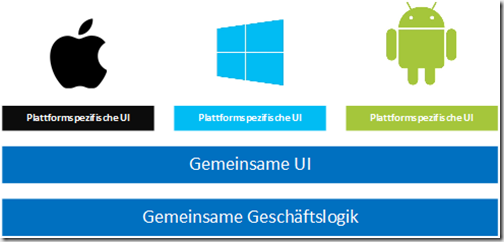
\includegraphics[scale = 0.5]{graphics/xamarin_forms-solution2.png}


\section{Fazit}
